\documentclass[10pt,twocolumn]{article}

\usepackage{geometry}
\geometry{a4paper}
%%\usepackage[cm]{fullpage}

%%\usepackage[top=2in, bottom=1.5in, left=2in, right=1in]{geometry}


\addtolength{\hoffset}{-25pt}
\addtolength{\textwidth}{35pt}


\usepackage{graphicx}
\usepackage{float}
\usepackage{wrapfig}

\linespread{1.} % Line spacing

\graphicspath{{figs/}}

\usepackage{polski}
\usepackage[utf8]{inputenc}

\DeclareFixedFont{\ttb}{T1}{txtt}{bx}{n}{8} % for bold
\DeclareFixedFont{\ttm}{T1}{txtt}{m}{n}{8}  % for normal
\usepackage{color}
\definecolor{deepblue}{rgb}{0,0,0.5}
\definecolor{deepred}{rgb}{0.6,0,0}
\definecolor{deepgreen}{rgb}{0,0.5,0}
\usepackage{listings}


% Python style for highlighting
\newcommand\pythonstyle{\lstset{
language=Python,
basicstyle=\ttm,
otherkeywords={self},             % Add keywords here
keywordstyle=\ttb\color{deepblue},
emph={MyClass,__init__},          % Custom highlighting
emphstyle=\ttb\color{deepred},    % Custom highlighting style
stringstyle=\color{deepgreen},
frame=tb,                         % Any extra options here
showstringspaces=false            %
}}
% Python environment
\lstnewenvironment{python}[1][]
{
\pythonstyle
\lstset{#1}
}
{}
% Python for external files
\newcommand\pythonexternal[2][]{{
\pythonstyle

\lstinputlisting[#1]{#2}}}

\lstset{language=Python}
% Python for inline
\newcommand\pythoninline[1]{{\pythonstyle\lstinline!#1!}}

\title{Rzut ukośny, czyli o prawie Newtona i równaniach różniczkowych}

\begin{document}

\maketitle
\begin{wrapfigure}[10]{l}[0cm]{4cm}
     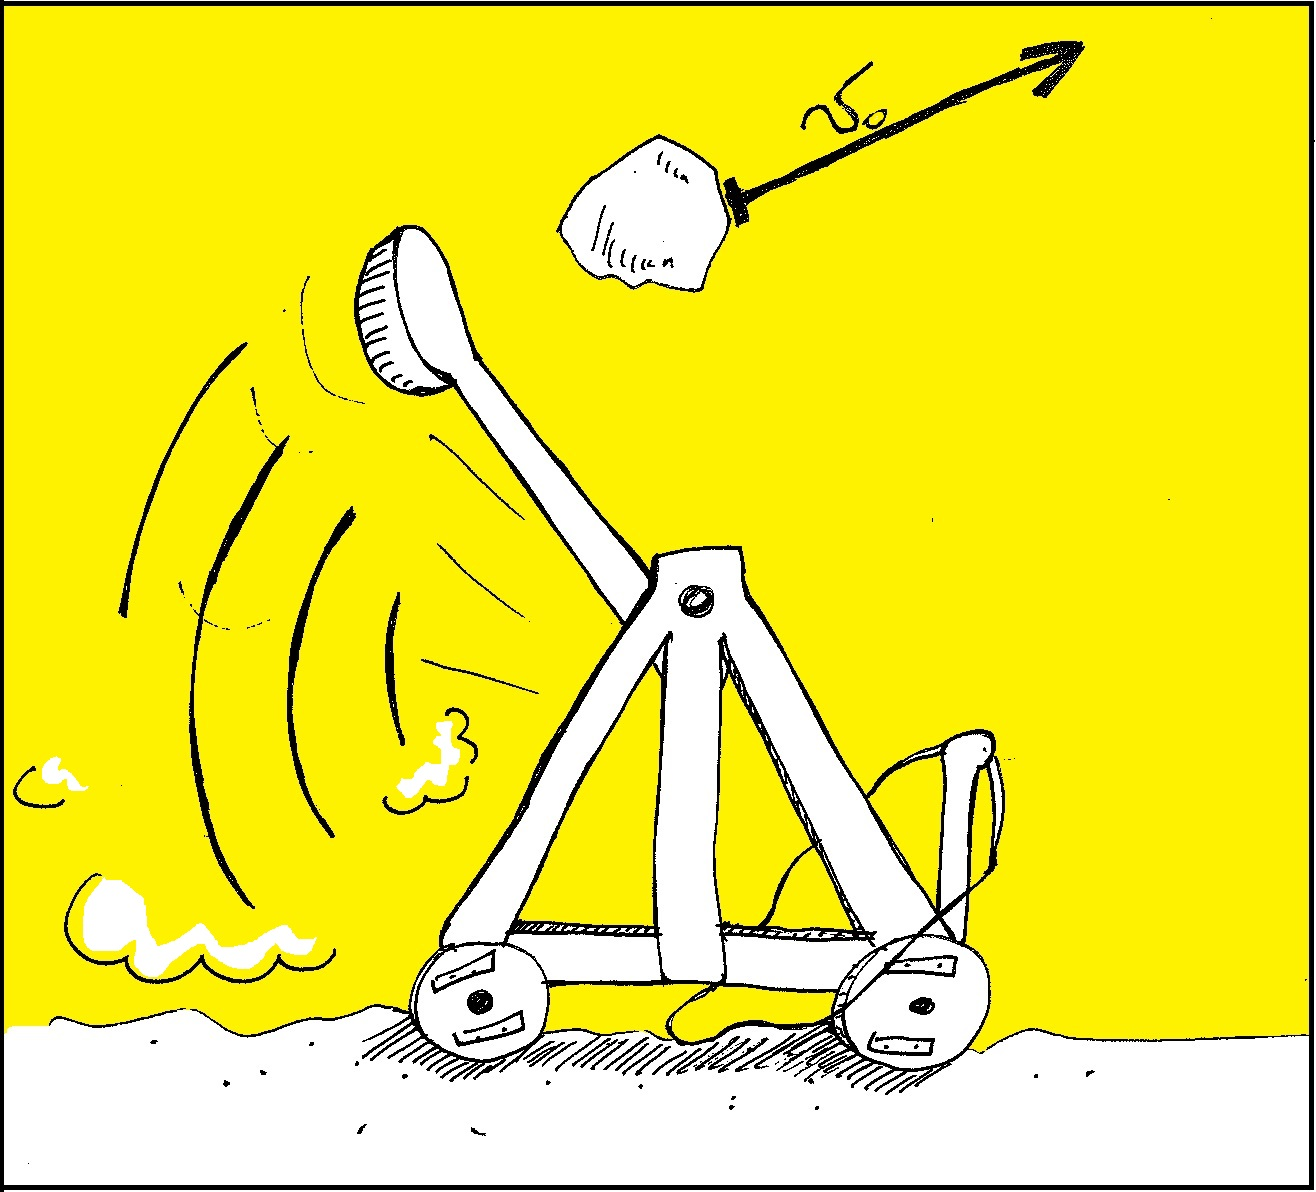
\includegraphics[width=4cm]{3.jpg}
\end{wrapfigure}



Z lekcji fizyki wszyscy wiemy, że prędkość cząstki $v=\frac{\Delta
  x}{\Delta t}$ opisuje tempo zmiany położenia $\Delta x$ w czasie
$\Delta t$. Z kolei przyspieszenie $a=\frac{\Delta v}{\Delta t}$
opisuje tempo zmiany prędkości $\Delta v$ w czasie $\Delta t$. Te
pozornie mało spektakularne wzory nabierają Mocy dopiero w zetknięciu
z komputerem. Czytelnika chcącego głębić tajniki metody rozwiązywania
równań różniczkowych zapraszamy do {\it aktywnej} lektury tego
artykułu.


Odkrywanie praw fizycznych przez ``komputerowe eksperymentowanie'' z
równaniami jest celem projektu dydaktycznego iCSE prowadzonego na
Uniwersytecie Śląskim. Narzędzie stanowi system Sage\ \cite{sagemath}
będący otwartą implementacją systemu algebry komputerowej z językiem
Python. Program Sage jest dostępny z poziomu przeglądarki internetowej
poprzez usługę chmurową\ \cite{cloud} lub serwer pojedyńczych obliczeń  na
którym bazuje interaktywna wersja tego artykułu\ \cite{web}.
%
 


\section{Rzut ukośny}

\begin{wrapfigure}[11]{l}[0cm]{5cm}
     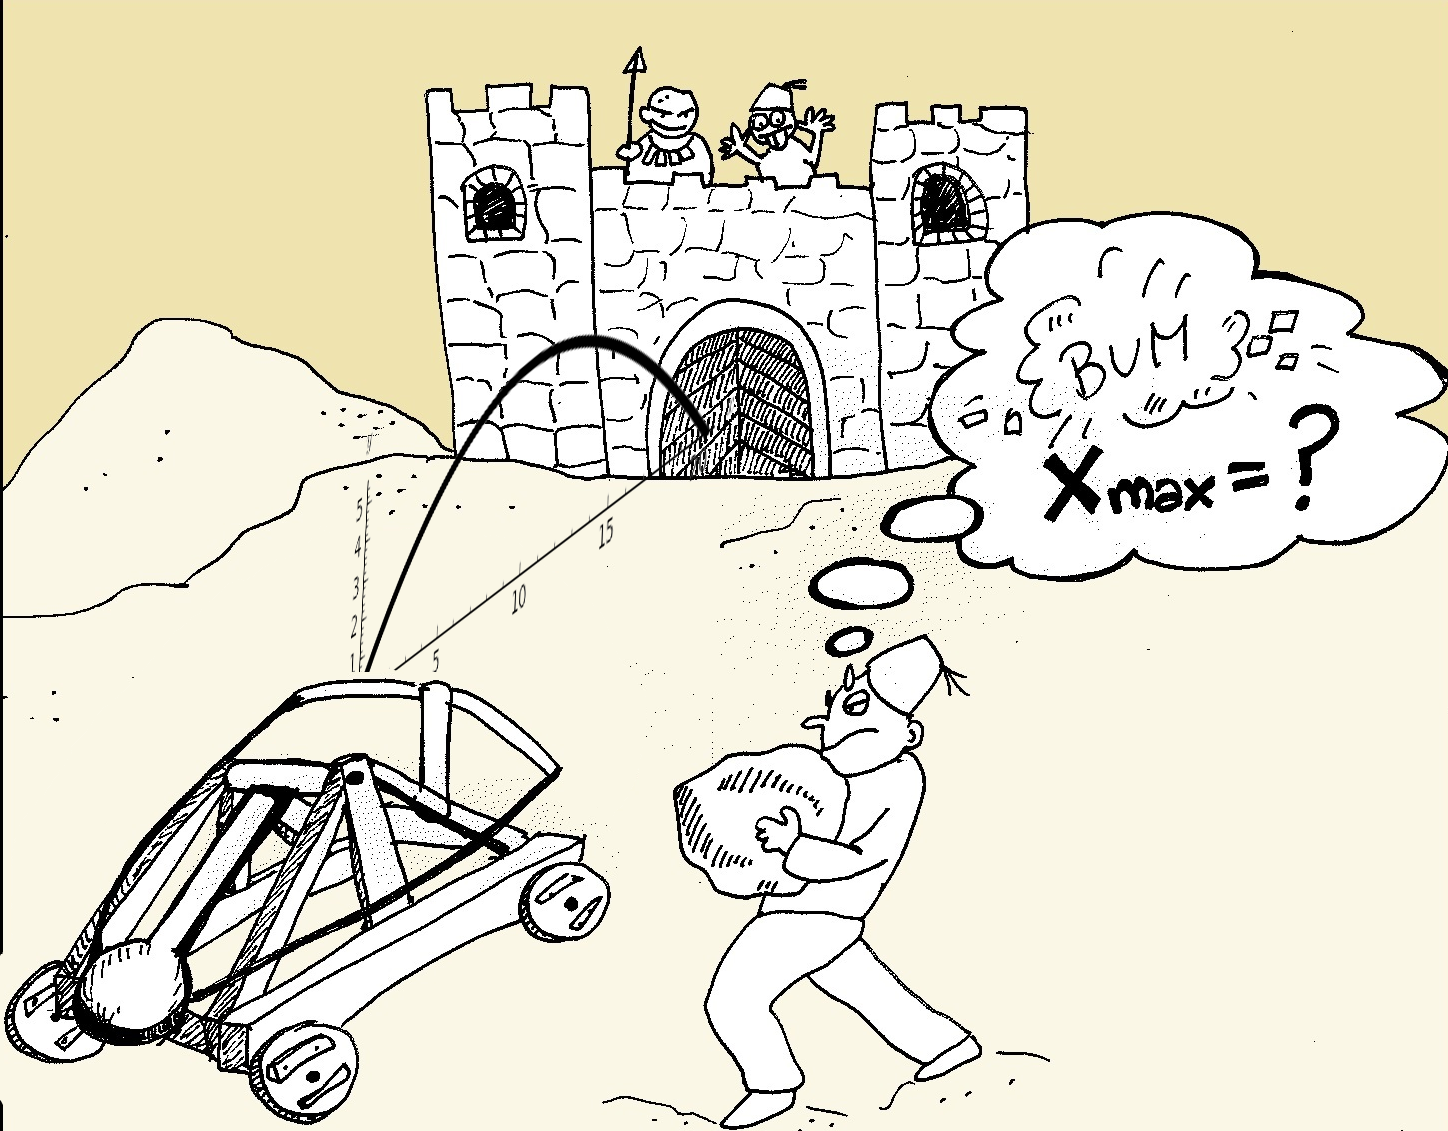
\includegraphics[width=5cm]{1a.png}
\end{wrapfigure}
Rozpoczniemy od pozornie nudnego tematu jakim może się wydawać znany
ze szkoły rzut ukośny. W fizyce pojęcie to oznacza ruch punktu
materialnego o pewnej masie pod działaniem siły grawitacji (siły
przyciągania ziemskiego). Wiedza na temat tego zagadnienia była
kluczowa podczas konfliktów zbrojnych. Wysyłając bowiem w stronę wroga
punkty materialne w postaci różnorakich pocisków, chcieliśmy wiedzieć
czy aby na pewno dotrą one do celu. Z tego punktu widzenia
interesujący jest zasięg posiadanego przez nas urządzenia miotającego,
oczywiście im większy tym lepszy. Można się spodziewać, że ów zasięg
zależy od siły miotającej naszego urządzenia, a co za tym idzie
prędkości początkowej pocisku. Kolejną rzeczą jest uwzględnienie kąta
wystrzału. Jeśli strzelimy pocisk pionowo to z pewnością upadnie na
nas - zasięg będzie zerowy. Jeśli strzelimy poziomo to również pocisk
nie poleci zbyt daleko. A zatem pod jakim kątem powinniśmy strzelać?
Odpowiedzi dręczące artylerzystów dostarcza Fizyka, a mówiąc
konkretnie jej gałąź zwana dynamiką. Rozwiązując więc odpowiednie
zagadnienie dynamiki dostajemy tor ruchu pocisku.

Podstawowym prawem jest słynna druga zasada dynamiki Newtona, która
wyraża się równaniem:

\begin{equation}
\label{eq:Ni}
m \vec  a = \vec F.
\end{equation}
%
W równaniu tym $m$ jest masą pocisku, $\vec a$ jest przyśpieszeniem
(wektorem o składowej poziomej i składowej pionowej) i $\vec F$ jest
siłą także o dwóch składowych: poziomej i pionowej.  Podczas lekcji z
reguły rozważa się przypadek, w którym pomijamy siły tarcia. Wówczas
jedyna siła działająca na ciało to siła o składowych $(0,-mg)$, tzn,
składowa pozioma wynosi 0, natomiast siła w kierunku pionowym wynosi
$mg$ i jest skierowana w dół (dlatego jest znak minus!). Możemy w
takim przypadku rozważać ruch odbywający się w płaszczyźnie rozpiętej
przez wektor siły i prędkości początkowej - czyli nasz pocisk będzie
leciał w płaszczyźnie pionowej do Ziemi i nie będzie skręcał w lewo
ani w prawo. Klasyczne rozwiązanie tego problemu oparte jest o fakt,
że ruch w poziomie $x$ i ruch w pionie $y$ są od siebie niezależne. W
kierunku pionowym ruch jest jednostajny, a w pionie zachodzi ruch
jednostajnie przyśpieszony. Można to zapisać w postaci
\cite{wikirzut}:
%
\begin{eqnarray}
\label{eq:param}
x(t) &=& x_0+v_{x0} t, \nonumber \\
y(t) &=& y_0 + v_{y0} t - \frac{1}{2}g t^2.
\end{eqnarray}

\noindent Równania (\ref{eq:param}) są tak zwanym parametrycznym
przedstawieniem toru ruchu. Oznacza to, że znamy jak w zależności od
parametru $t$ (czyli czasu) zmienia się każda ze współrzędnych $x$ i
$y$. Wyliczając czas $t$ z pierwszego równania i wstawiając go do
drugiego równania można przekształcić te dwa równania do postaci
funkcyjnej $y=f(x)$. Otrzymamy wtedy równanie paraboli o ujemnym
współczynniku przy wyrazie $x^2$. Jednak w programie Sage mamy bardzo
wygodną procedurę do rysowania właśnie takich krzywych parametrycznych
- mianowicie funkcję \verb|parametric_plot|.

\pythonexternal{code01.py}

Rysownie tych krzywych jest fajną zabawą! Wyobraźmy sobie, że armata
ma funkcję działa przeciwlotniczego i pytamy się w jakim obszarze
przestrzeni jej pociśki mogą dosięgnąć wrogi samolot?
\begin{wrapfigure}[8]{l}[0cm]{4cm}
     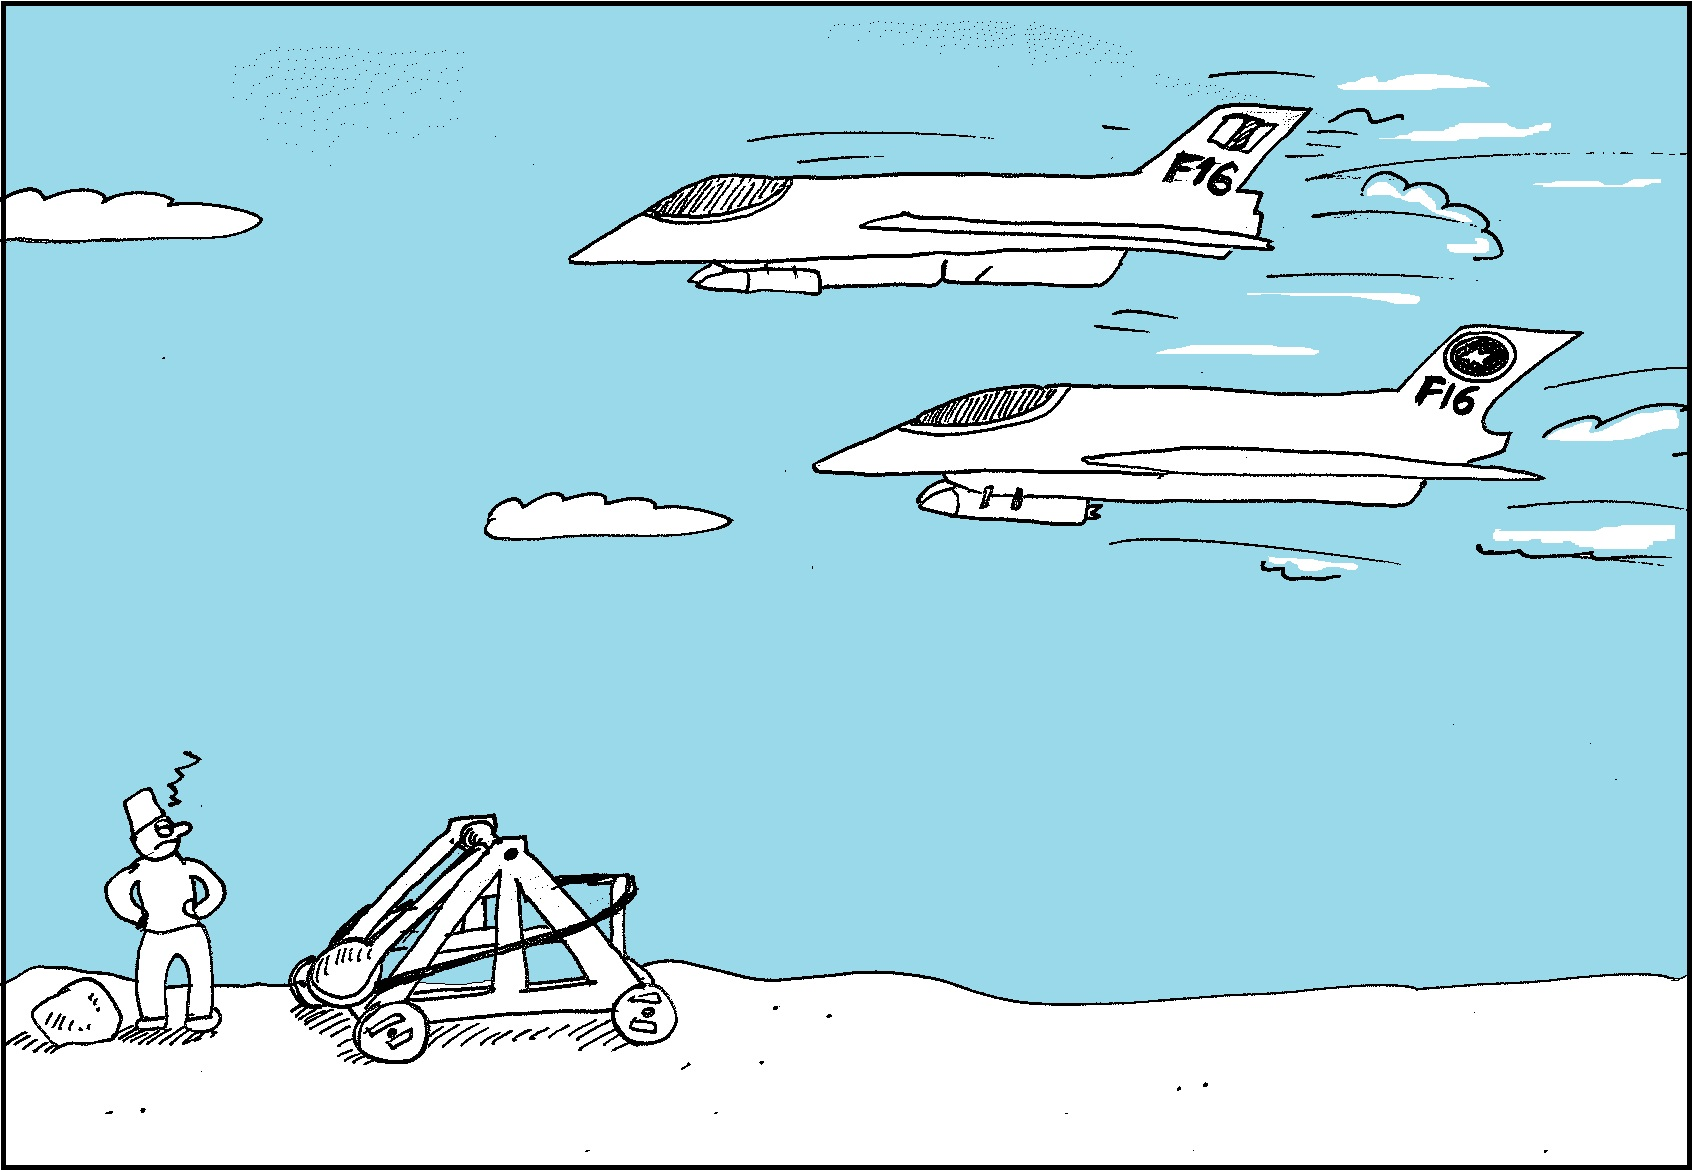
\includegraphics[width=4cm]{2.jpg}
\end{wrapfigure}
Narysujmy w Sage na jednym wykresie tory wystrzałów z prędkościami
$v_{x0}=v_0 \cos(\alpha)$ i $v_{y0}=v_0 \sin(\alpha)$, dla różnych
kątów $\alpha$ (to jest kąt pomiędzy poziomem i wektorem prędkości
początkowej pocisku). Zachęcamy do samodzielnego napisania kodu, który
powinien generować coś zbliżonego do rysunku (\ref{fig:rzut1}).
%
\begin{figure}
    \begin{center}
     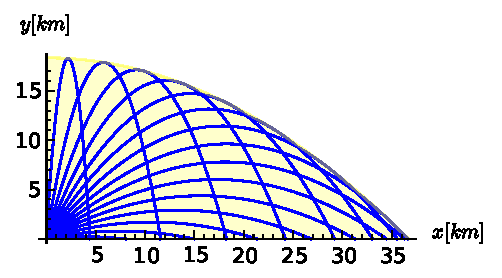
\includegraphics{pplot.pdf}
  \end{center}
  \caption{Obszar rażenia działa o prędkości początkowej pocisku $v_0=600m/s$. 
    \label{fig:rzut1} }
\end{figure}
%
Brzeg obszaru skutecznego ognia działa przeciwlotniczego, jest
matematycznie rzecz biorąc obwiednią rodziny krzywych. Nasz rysunek
sugeruje, że ma on kształt paraboli - i dokładny rachunek pokazuje, że
tak jest rzeczywiście (zob. \cite{web}).


\section{Rzut ukośny - inaczej}

Czytelnik pewnie zastanawia się, czy przypadkiem nie chcemy wrobić go
w przerobienie lekcji fizyki pod pretekstem rysowania wykresów funkcji
na komputerze. Otóż nie! Rozwiązanie matematyczne przyda się nam do
weryfikacji wyników rozważań nieco odmiennych niż te prezentowane
zazwyczaj w szkole. Rozważania te umożliwią nam analizę toru lotu
pocisku z uwzględnieniem bardziej realistycznych czynników takich jak
tarcie, wiatr czy nawet rotacja pocisku.

W równaniu Newtona dla ruchu pocisku występuje przyśpieszenie.
Oznaczmy przez $t$ pewną chwilę czasu, a przez $\Delta t$ mały
przyrost czasu. Dla składowej poziomej przyspieszenia otrzymujemy
relację
%
\begin{equation}
a_x = \frac{\Delta v_x}{\Delta t}=\frac{v_x(t+\Delta t)-v_x(t)}{\Delta t}. 
\label{eq:dv} 
\end{equation}
%
Z prawa Newtona dla składowej $x$-owej mamy:
%
\begin{equation}
a_x = \frac{F_x}{m}
\label{eq:dv} 
\end{equation}
%
więc możemy napisać 
%
\begin{equation}
\frac{v_x(t+\Delta t)-v_x(t)}{\Delta t} = \frac{F_x}{m}.
\label{eq:dv3} 
\end{equation}
%
Załóżmy, że znamy prędkość $v_x(t)$ w chwili $t$. Chcielibyśmy
obliczyć prędkość $v_x(t+\Delta t)$ w chwili $t+\Delta t$.  Z równania
(\ref{eq:dv3}) wynika, że

\begin{equation}
v_x(t+\Delta t) =v_x(t) + \Delta t\cdot  \frac{F_x}{m}.
\label{eq:euler1} 
\end{equation}
  
Świetnie! Zapiszmy podobne wzory dla składowej pionowej  i będziemy
mogli obliczać prędkość w dowolnej chwili czasu. A co z położeniem?
Możemy postąpić podobnie, stosując wzór na prędkość. I tak np. dla $x$:
\begin{equation}
  v_x = \frac{x(t+\Delta t)-x(t)}{\Delta t}
\label{eq:dx}  
\end{equation}
czyli
\begin{equation}
x(t+\Delta t)= x(t)+ \Delta t \cdot v_x 
\label{eq:euler2}
\end{equation}
%
Wzory (\ref{eq:euler1}) oraz (\ref{eq:euler2}) oraz odpowiedniki dla
składowych pionowych $y$ układają się w algorytm, który możemy
zaprogramować na komputerze. Ale chwileczkę...

Czy te wzory są poprawne? Niestety nie! W rów.  (\ref{eq:euler1})
założyliśmy prawo dla ruchu jednostajnie przyśpieszonego, a siła w
ogólności nie musi być stała. W rów.  (\ref{eq:euler2}) założyliśmy,
że prędkość jest stała, a nie musi wcale tak być. No chyba, że $\Delta
t$ jest odpowiednio małe. Wtedy można by się spodziewać, że siła i
prędkość w czasie między $t$ a $t+\Delta t$ nie zmienią się. Wówczas wzory byłyby przybliżeniem prawdy. Sprawdźmy to
eksperymentalnie wykonując poniższy kod w systemie Sage:

\pythonexternal{code02.py}

\noindent Podobnie jak w przypadku rysowania rozwiązania dokładnego
startujemy z zadania warunków początkowych i parametrów układu (linie
1-3). Następnie zakładamy, że chcemy zastosować przybliżoną procedurę
$n=200$ razy w ciągu całego  lotu pocisku. Wyliczamy $\Delta
t=t_{end}/n$ (linia 6). Wykonujemy $n$ razy pętlę w której korzystamy
z czterech przybliżonych wzorów (\ref{eq:euler1}),(\ref{eq:euler2}) i
analogicznych dla komponentu pionowego. Linia 12 jest niezwykle ważna
bowiem ``ustawia'' wyliczone nowe wartości prędkości i położenia jako
warunki początkowe dla kolejnego kroku. W linii 13 dołączamy wybrane
parametry - akurat interesuje nas położenie - do listy punktów
potrzebnych do późniejszego narysowania (dwie ostatnie linie) toru
pocisku. Jeżeli w tej samej sesji Sage wykonaliśmy już pierwszy
program, to możemy łatwo narysować rozwiązanie dokładne i przybliżone
na jednym wykresie komendą: \verb|(p1+p2).show()|.
%
\begin{figure}
    \begin{center}
     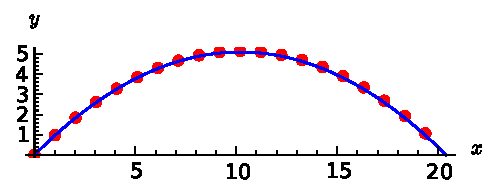
\includegraphics{porownanie.pdf}
  \end{center}
  \caption{Porównanie wyniku dokładnego i metody numerycznej.
    \label{fig:por} }
\end{figure}
%

Na rysunku \ref{fig:por} widzimy, że otrzymaliśmy tor ruchu zbliżony
do dokładnego. Zachęcamy Czytelnika do samodzielnych eksperymentów i
zbadania jak np. ilość iteracji - czyli krok czasowy - wpływa na
wynik. Ciekawostką jest, że nasz program nigdzie nie zawierał funkcji
kwadratowej, a pomimo tego narysował jej wykres - parabolę!
 
Po co robiliśmy tyle szumu i zaprzęgali komputer do obliczania tego co
było i tak znane?  Przecież w przypadku rzutu ukośnego metoda
numeryczna z mozołem odtwarza wynik analityczny. Okazuje się, że nasz
algorytm może być użyty do rozwiązywania praktycznie KAŻDEGO
zagadnienia opisanego równaniem Newtona! Wystarczy zmodyfikować
wyrażenia dla sił. Co więcej, siły  mogą zależeć w najdziwniejszy sposób od
każdej ze zmiennych. Wystarczy w naszym algorytmie zmienić zaledwie
dwie linie:

\pythonexternal{code03.py}
% 
\noindent gdzie za $F_x,F_y$ wstawiamy odpowiednie wyrażenia na siły w kierunku poziomym i pionowym,
które chcemy modelować. Na przykład możemy rozwiązać układ,  w którym
mamy realistyczną siłę oporu, która zależy kwadratowo od
prędkości. Możemy dodać wiatr i to nawet taki, który wieje inaczej na wysokości 
100m nad Ziemią,  a inaczej na wysokości 10km. Możemy uwzględnić zmianę gęstości
powietrza na dużych wysokościach. W takich przypadkach nie jest łatwo
lub wręcz się nie da otrzymać rozwiązania metodami analitycznymi.

Cierpliwych Czytelników zapraszamy do lektury następnej części tego
artykułu. Niecierpliwych zachęcamy do samodzielnego eksperymentowania
od zaraz.
 
\section{A równania różniczkowe?}

Czyżby dopadła nas cyfrowa demencja - przecież mieliśmy się dowiedzieć czegoś  o równaniach różniczkowych! 
Okazuje się, że nasz drugi program tak na prawdę był schematem Eulera
rozwiązującym układ czterech równań różniczkowych zwyczajnych!  Skoro
potrafimy już je rozwiązywać, to może dowiedzmy się co to jest?
Mówiąc mniej precyzyjnie, jest to równanie podobne do (\ref{eq:dv3}),
ale w granicy $\Delta t\to0$. Lewa strona przechodzi w wielkość zwaną
pochodną (w tym przypadku pochodną prędkości). Równania różniczkowe to
właśnie takie równania, które zawierają funkcje (w naszym przypadku
$x(t),v_x(t),y(t),v_y(t),$ i ich pochodne. Przybliżając granicę przez
wzięcie pewnego małego, ale skończonego $\Delta t$ otrzymaliśmy
właśnie schemat numeryczny rozwiązujący nasze równania różniczkowe.

\begin{thebibliography}{1}

\bibitem{sagemath} http://sagemath.org
\bibitem{cloud} http://cloud.sagemath.com
\bibitem{web} http://visual.icse.us.edu.pl/Warsztaty
\bibitem{wikirzut} http://pl.wikipedia.org/wiki/Rzut\_ukośny

\end{thebibliography}

\end{document}

